%==============================================================================
% Document:    
% File:        
% Authors:     
%==============================================================================


%==============================================================================
% Document setup
%==============================================================================

\documentclass[12pt,a4paper]{report}


% Use packages
\usepackage{stys/kiss}
\usepackage{verbatim}
\usepackage{rotating}
\usepackage{color}
\usepackage{a4}
\usepackage{url}
\usepackage{stys/enumerate}
\usepackage{graphicx}
\usepackage{stys/moreverb}
\usepackage{xcolor}
\usepackage[anchorcolor=black,bookmarksnumbered=true,bookmarksopen=true,linkcolor=black,menucolor=black,pagecolor=black,linkbordercolor={1
1 1}]{hyperref}
\usepackage{stys/placeins}
\usepackage{stys/longtable}
\usepackage{caption2}
\usepackage{stys/lipsum}

% Specify document wide settings/parameters
\setcounter{secnumdepth}{5}
\setcounter{tocdepth}{1}
\setlength{\parindent}{0cm}
\setlength{\parskip}{1.5ex plus 0.5ex minus 0.2ex}


% Include the LaTeX definitions of commonly used terms
% ====================================================
% Definitions of terms/abbreviations used in the LaTeX document.
% Not to be confused with document glossary/data dictionary
% ====================================================

\def \csse  {Department of Computer Science and Software Engineering}
\def \UoM  	{University of Melbourne}
\def \team	{Adam Whiteside, Andrew Vadnal, Scott Richie and Terence Signakis}
\def \subjname {COMP90024 (433678): Cluster and Grid Computing}

% ====================================================
% Definitions of new commands/environments
% ====================================================
% For displaying the usage of the UNIX command line tools
\newcommand{\cmdusage}[1]{%
            {\tt{#1}}}

% For displaying the name of a UNIX command line tool
\newcommand{\cmd}[1]{%
            {\texttt{#1}}}

% For showing definitions and acronyms
\newcommand{\introdef}[2]{%
            {\item \textbf{#1:} #2}}

% For highlighting the first word in an enumeration
\newcommand{\point}[1]{%
            {\item \textbf{#1:}}}

% For attributes of objects
\newcommand{\attr}[1]{%
            {\emph{#1}}}


%\def \movemousecursor{R1.1 Mouse Movement}


% Document revision/release number
\def \revision  {0.1}
\def \vdate {\today}
\def \authors {Terence Siganakis (134860),
Scott Ritchie (330975),
Andrew Vadnal (326558), and
Adam Whiteside (327705)}

\addtolength{\oddsidemargin}{-.2in}
\addtolength{\evensidemargin}{-.2in}
\addtolength{\textwidth}{.5in}

\addtolength{\topmargin}{-.7in}
\addtolength{\textheight}{1.3in}



%==============================================================================
% Begin document content
%==============================================================================
\begin{document}
\begin{titlepage}
\begin{center}
\begin{figure}[h]
	\begin{center}
    	
\includegraphics[height=45mm]{figs/UOM_logo.pdf}
	\end{center}
\end{figure}

\Large\rmfamily{Department of \\ Computer Science and Software Engineering} \\
\vspace*{35mm}
\huge\sffamily{Term Paper}\\
\vspace*{5mm}
\large\sffamily{for}\\
\vspace*{5mm}
\Huge\sffamily{~\subjname~}\\
\vspace*{20mm}
\Large\rmfamily{Version: \revision} \\
\small{\vdate}\\

\vspace*{40mm}
\begin{quotation}
	\noindent
The purpose of this document is to...
\end{quotation}

\end{center}
\end{titlepage}
\pagestyle{plain}
\pagenumbering{roman}

% ========================
% Inside cover page
% ========================      
% vim: ts=4 sw=4 expandtab textwidth=72
% ====================================================
% The inside cover page, including items like copyright, authors, etc
% ====================================================


\subsection*{Copyright notice}

Copyright \copyright~2012, \authors.
Permission is granted to reproduce this document for internal \team~use only.

\begin{figure}
	\begin{flushleft}
    	
\includegraphics[height=35mm]{figs/UOM_logo}
	\end{flushleft}
\end{figure}
\csse\\
The \UoM\\
Victoria\\
AUSTRALIA\\
3010\\
\\
ICT Building\\
111 Barry Street\\
Carlton\\
\\
Tel: +613 8344 1300\\
Fax: +613 9348 1184\\
\url{http://www.csse.unimelb.edu.au/}\\

Version: \revision \\
\vdate. \\



\subsection*{Credits}

This document was written by \authors.


\newpage


% ========================
% Table of contents, list of figures
% ========================      
\tableofcontents                   
%\listoffigures                   
\newpage
\pagenumbering{arabic}

% ============================
% Start of main body of the document
% ============================

% Azure footnotes:

\newcommand{\ftAone}[0]{\footnotemark[1]}
\newcommand{\ftAoneText}[0]{
\footnotetext[1]{Windows Azure. \emph{Home Page}, Retrieved May 14, 2012. http://www.windowsazure.com/en-us/}
}

\newcommand{\ftAimg}[0]{\footnotemark[2]}
\newcommand{\ftAimgText}[0]{
\footnotetext[2]{Temi Odurinde. \emph{Windows Azure -- Microsoft Clouds Computing}, Retrieved May 14, 2012. http://www.temi.co.uk/windows-azure-microsoft-clouds-computing/}
}

\newcommand{\ftAtwo}[0]{\footnotemark[3]}
\newcommand{\ftAtwoText}[0]{
\footnotetext[3]{Wikipedia. \emph{AppFabric}, Retrieved May 14, 2012. http://en.wikipedia.org/wiki/AppFabric}
}

\newcommand{\ftAthree}[0]{\footnotemark[4]}
\newcommand{\ftAthreeText}[0]{
\footnotetext[4]{GigaOM. \emph{Everything You Need to Know About Microsoft Azure}, Retrieved May 14, 2012. http://gigaom.com/2009/07/14/microsoft-azure/}
}

\newcommand{\ftAfour}[0]{\footnotemark[5]}
\newcommand{\ftAfourText}[0]{
\footnotetext[5]{Windows Azure. \emph{Windows Azure Storage}, Retrieved May 14, 2012. http://www.windowsazure.com/en-us/home/features/storage}
}

\chapter{Introduction}
Over the course of the last decade outsourcing the delivery of computational
resources to external companies has become more and more popular for personal,
business and scientific uses. In a manner analogous to water, gas and
electricity, computing power can be treated as a resource and charged based on
individual usage~\cite{Aneka}. This delivery of computing resources as a
service over the Internet is known as Cloud computing. 

Cloud computing has a number of benefits for end users wishing to access and
use external resources:
\begin{itemize}
\item Resources can be accessed from anywhere; users are no longer tied down to their machine in a physical location.
\item Users do not have to maintain their own hardware, other than a machine to act as a portal to these utilities.
\item Users are able to access much greater computing resources than would otherwise be available to them.
\item Users no longer have to worry about losing data if their machine fails as it is distributed across the Cloud.
\end{itemize}

\section{Cloud Computing Architecture}
Cloud computing can deliver services to both end users and developers. These
services extend to a number of different levels, providing resources which are beneficial to all types of users.~\cite{Aneka}:
\begin{itemize}
\introdef{Software as a Service (SaaS)}{Individual applications which make use of the cloud for either storage of computing power.}
\introdef{Platform as a Service (PaaS)}{A platform for development across a distributed network of machines is provided to the end user.}
\introdef{Infrastructure as a Service (IaaS)}{Off-site hardware infrastructure is provided to a number of end users to securely access and use for their own purposes.}
\end{itemize}

In this report we will be focusing on the PaaS and IaaS services available to developers, rather than looking at SaaS solutions. 

\chapter{Related Works}
In this report four cloud computing services are examined; Google App Engine, Microsoft Azure, Amazon EC2, and Manjrasoft Aneka. Each of these offers a different type, and level of services to developers to run applications on the cloud.

\begin{table}[h]
\centering
\begin{tabular}{|p{2.5cm}||p{3cm} p{3cm} p{5cm}|}
\hline 
\textbf{Name} & \textbf{Description} & \textbf{Remarks} & \textbf{URL}\tabularnewline
\hline 
\hline 
\textbf{Google App Engine} & Google App Engine is a PaaS which allows developers to develop and deploy web applications on Google's Infrastructure & PaaS \& IaaS & \small{http://appengine.google.com/}\tabularnewline
\textbf{Microsoft Azure} & Compute (Web Applications) & Compute & dafs \tabularnewline
\textbf{Amazon EC2} & Web Applications & Azure Services & Customisable VM\tabularnewline
\textbf{Manjrasoft Aneka} & Automatic & Automatic & Manual\tabularnewline
\hline
\end{tabular}
\caption{Description of cloud computing services}
\end{table}

\newcommand{\gae}[0]{Google App Engine}
\newcommand{\mr}[0]{\emph{MapReduce}}
\chapter{Google App Engine}

\section{Description}
\gae{} is a Platform as a Service cloud computing environment provided by Google which allows developers to develop and deploy distributed web applications on Google's infrastructure. This platform abstracts all notion of parallelism away from the developer. Google takes care of all the parallelism behind the scenes while guaranteeing a fast, scalable environment for developers to work in. 
%cite PaaS http://arxiv.org/pdf/0907.4622.pdf

While Google is secretive about the underlying architecture of its servers, \gae{} is most likely deployed across Google's servers using some variation of \mr{}. Developed in the late 1990s, \mr{} is a method for distributing programming tasks across multiple processes. MapReduce is based on functional programming paradigms, specifically the \emph{Map} and \emph{Reduce} functions typically found in such languages. Developers supply a list of data, and a function to apply to that data. This is the \emph{Map} step in \mr{}. Another function is also provided by the developer, to be used in the \emph{Reduce} step, which combines the resulting list of data to obtain the final result. All parallelism is handled by \mr{}, abstracting all notion of parallel programming away from application development. This is \mr{}'s strength and what allows Google to provide guaranteed automatic scaling to users of \gae{}.

% Map Reduce Scheduling: (Can be used in final report for comparison)
%
% 	- Highly fault tolerant. When Jobs fail, reassigns to another idle node.
%	- atomic commits
%	- Straggler nodes
%		- When MapReduce near completion, schedules backup executions of final in-progress job(s). Completes whenever primary or backup completes
%		- takes 44\% longer to complete when disabled.
%	- Combiner function can be specified that does partial merging on worker nodes before being sent to the network

\begin{center}
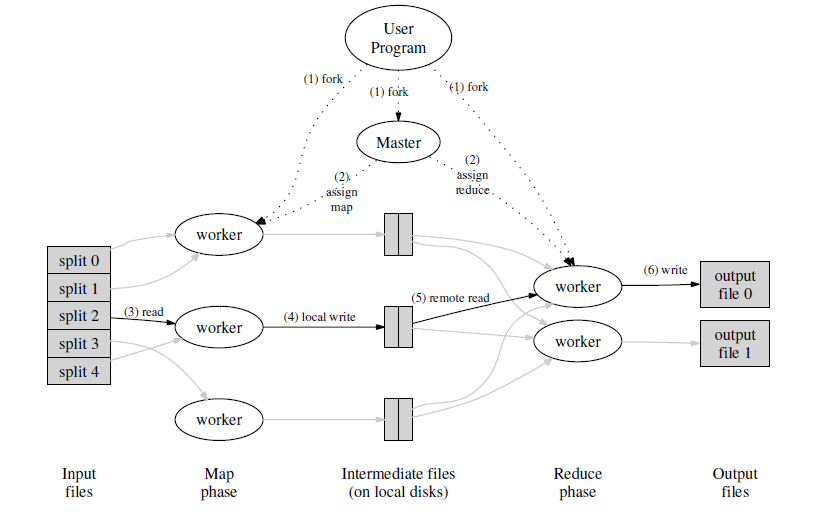
\includegraphics[scale=0.4]{figs/MapReduce.png} \\
\texttt{Overview of MapReduce execution} % Citation %
\end{center}

\section{Application Runtime Environment}
\gae{} provides three runtime environments to develop and deploy applications in; Python (2.5.2 and 2.7.2), Java (SDK 5 or 6), and Google's own language, Go (experimental). Developers can also use other JVM based languages such as Ruby and JavaScript in the Java runtime environment. A local development environment which emulates \gae{} is also provided. 

These are not the standard runtime environments typically used for development in these languages. Google provides a restricted version of the respective standard libraries, allowing google to effectively scale and sandbox the runtime environments. The restrictions to the standard libraries are as follows:
\begin{itemize}
\item Computers can only connect to \gae{} over HTTP(S) on standard ports.
\item No filesystem access.
\item Applications can only access other computers using Google's provided web services.
\item Code can only run in response to a web request, queued task or scheduled task. 
\item Applications must take no longer than 60 seconds to respond to a request.
\end{itemize}

In addition to this restricted standard library, Google also provides a number of services:
\begin{itemize}
\item APIs for authenticating users through Google Accounts.
\item An admin console for mantaining existing applications
\item Image manipulation
\end{itemize}

\section{Data Storage}
While Google restricts the standard libraries of its runtime environments to prevent reading and writing to file, two main methods are provided for persisent concurrent data storage; Memcache and the Datastore.

\subsection{Memcache}
Memcache is a service provided by Google which provides a high performance, in memory key-value store. This is stored in cache and can be accessed across multiple instances of an application.

\subsection{Datastore}
One of \gae{}'s features is its automatically scaling datastore, a database-like system which allows for persistent storage within an application. The Datastore is a NoSQL schemaless object datastore, allowing for persistent storage of Objects. 

Objects in the datastore are entities with a \emph{kind} and a set of a properties. Using Java as an example, objects can be persistently stored in the datastore; the class is the entity's \emph{kind} and its properties are the object's attributes. These can be stored and accessed using either JDO or JPA's persistence managers and query engines.

The Datastore is based on the \emph{High Replication Datastore} design: a system based on the \emph{Paxos algorithm} is used to replicated data across multiple servers. The datastore is strongly consistent and uses optimistic concurrency control. This means that transactions can proceed without locking because it assumes that multiple transactions can be completed without affecting each other. When a commit is made to the datastore each transaction checks that no others have modified the relevant part of the datastore since the transaction started. If changes are found, the commiting transaction is rolled back.
 
\subsection{External Services}
While the datastore is automatically scalable and provides high performance, it does not guarantee, and in some cases allow for atomic transactions where relations between objects exist. Some situations require relational algebra, so Google also provides access to its relational SQL database service known as \emph{Cloud SQL} from within \gae{}. 

Google also provides access to its \emph{Cloud Storage} system, which allows for storage of files up to a terabyte in size. This however cannot be accessed from the Google Go runtime environment.

\section{Cost}
\gae{} can be used for free, giving any developer 1 GB of storage and up to 5 million page views a month. Once either of these limits are exceeded service to an application will be cut off for that month unless billing options are implemented. Pricing for \gae{}'s services is complex, containing varying costs for reads/writes to the datastore and hours per instance required. These can be found at \emph{https://developers.google.com/appengine/docs/billing}. A minimum of \$2.10 per week must be spent if the billable services are used, and developers can specify a maximum daily budget.

\chapter{Microsoft Azure}
Microsoft Windows Azure can be perceived as an operating system provided to users by a service. This ensures that Azure can be used from anywhere, providing that the OS is hosted on a Microsoft-based cloud. Officially released on the 1st of February 2010, the Microsoft Windows Azure software is a cloud computing platform on which web applications can be readily built (using languages such as Java and Python, and frameworks such as .NET and Ruby on Rails), hosted and scaled across the globally spanning network of Microsoft hosted data centres. On-demand services are also hosted on these data centres, notably Windows Azure\ftAone\ftAoneText, SQL Azure and Windows Azure AppFabric. The following figure displays a high level architectural outline of the Azure cloud:

\begin{center}
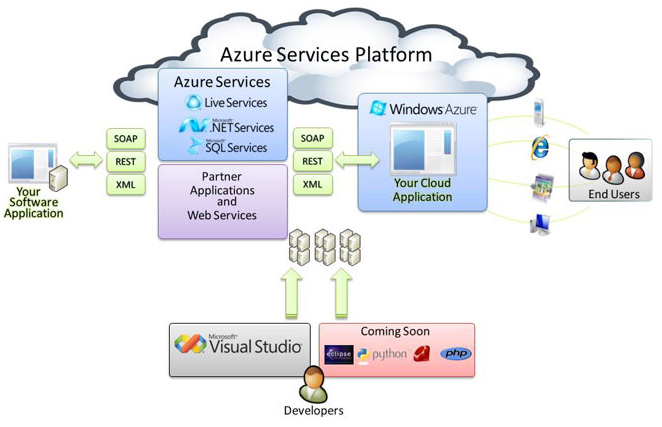
\includegraphics[scale=0.8]{figs/Azure.png} \\
\texttt{High level architectural outline of the Azure cloud}\ftAimg\ftAimgText
\end{center}

Windows Azure is an OS that facilitates both application hosting and data storage. It is upon these two services that users will build and maintain their products once an Azure subscription has been purchased. SQL Azure is a scaled, cloud based implementation of Microsoft SQL Server -- a relational database server and Windows Azure AppFabric represents a collection of cloud computing services at the middleware level.

Notable services are included within AppFabric include, but are not limited to\ftAtwo\ftAtwoText:
\begin{itemize}
\item Access Control Service -- Controls user authorisation on related services and applications.
\item Service Bus -- Ensuring that secure connections are in place on cloud-based applications.
\item Caching -- Allows applications to utilise the high-speed caching service provided by the Microsoft cloud; ensuring a high access time to application data.
\end{itemize}

The implementation of rigorous security measures are of critical importance, particularly within a cloud-based service which is available to consumers on a global scale. When users subscribe to the Azure cloud, the credit card used to transfer funds is associated to the user making the payment. In addition, access to the cloud service is performed via signing in through a Windows Live ID account. 
There are three pricing packages\ftAthree\ftAthreeText in place for the Azure cloud service. These packages include:
\begin{itemize}
\item Consumption-based -- Costs are incurred only when data is used.
\item Subscription-based -- Committing to a fixed price over a specified number of months.
\item Volume-based -- Tailored for large organisations that already possess at least one Microsoft licence -- allowing for these services to be integrated into the Microsoft cloud. 
\end{itemize}

Once a consumer has signed up to the Azure cloud, enforcing a secure means of user authentication is paramount to the security of any stored data. In order to differentiate between application hosting and data storage, Windows Azure uses separate methods used to authenticate users to each service. These methods are outlined in the following table~\cite{AzureSecurity}:

\begin{center}
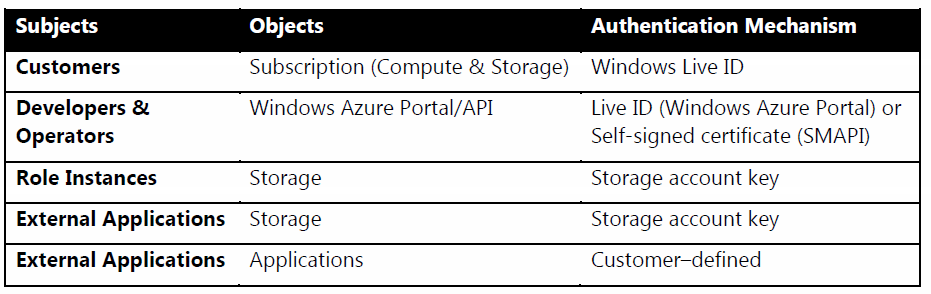
\includegraphics[scale=0.6]{figs/AzureTable.png} \\
\end{center}

Accessing applications hosted on the Azure cloud can be performed by two methods: via the Windows Azure website itself or via the Service Management API (SMAPI). The latter requires the registration of a public/private key and a self-signed certificate associated to each user utilising the cloud service when uploading developed applications. SMAPI authentication references the aforementioned key pair and user certificate before each user session can commence.

When accessing stored content on the Azure cloud, users require an account-specific Storage Account Key (SAK). This key is able to be changed at any time.

The Windows Azure platform must provide fundamental security concepts on its cloud service, in order for consumers to acknowledge that their data is stored safely on the Microsoft cloud. Confidentiality, integrity, availability and accountability are the terms used to describe how security is approached on the Azure platform. Notable features pertaining to each of these terms are as follows~\cite{AzureSecurity}:

\begin{itemize}
\item Confidentiality
\begin{itemize}
\item Encryption -- Used internally within Windows Azure for protecting control channels and is provided optionally for customers who need rigorous data protection capabilities. 
\end{itemize}
\item Integrity
\begin{itemize}
\item Each Virtual Machine (VM) is connected to three local Virtual Hard Drives (VHD)
\begin{itemize}
\item The first VHD contains one of several versions of the Guest OS. The consumer selects the new patches they wish to apply, ensuring that the OS is always at the most recent version.
\item The second VHD contains an image constructed by the Fabric Controller (FC).
\item The last VHD contains configuration data, all paging files and storage. 
\end{itemize}
\end{itemize}
\item Availability \\ The Azure platform ensures that stored data will not be compromised by employing rigorous backup techniques. These techniques include, but are not limited to\ftAfour\ftAfourText:
\begin{itemize}
\item Data replication -- replicating data three times in the same data centre as a precaution against hardware failure – in turn ensuring that data is always available.
\item Geo-replication -- Data is replicated between data centres that are not situated within geographic vicinity. This approach safeguards against any natural disasters.
\end{itemize}

Adopting the Microsoft Windows Azure software is a viable solution for both a personal or business need to utilise a distributed cloud computing service to store and maintain developed applications. As with moving towards any new software, it is up to the consumer to adequately research many factors such as cost, security, data storage capabilities and data availability when making use of a cloud based hosting service. The consumption and subscription based pricing packages are ideal for consumers who are both unsure of how much data they will need and consumers who wish to move to the Microsoft cloud for a defined month period.

\end{itemize}

\chapter{Amazon EC2}

\chapter{Aneka}
\section{Introduction}
Aneka is a Platform-as-a-Service (PaaS) that enables the development of distributed applications for use across a broad range of cloud, grid and cluster platforms. Originally developed as part of the Gridbus Project, Aneka was later commercialised by Manjirasoft and is developed on top of .NET technology. It is available freely for a trial period[4], however additional arrangements must be made for commercial use. Aneka allows for applications to be developed in any language that is supported by the .NET runtime, such as VB.NET and C\#, and through the use of Mono, allows applications to run on Linux and OSX as well as Windows infrastructures\cite{Aneka}.

\section{Platform as a Service}
PaaS solutions, such as Aneka, provide a platform from which distributed applications can be developed that scale on demand\cite{CloudBus}. Aneka is a pure PaaS in that it does not provide an underlying hardware infrastructure. This differs from other PaaS solutions such as Google AppEngine and Microsoft Azure, which are both PaaS and Infrastructure-as-a-Service (IaaS) solutions. Instead, Aneka is designed to work as a platform layer on top of a variety of infrastructures, including combinations of multiple different options. This allows for the use of local resources when available, with the added ability for the provision of additional cloud resources from a service such as Amazon EC2 when the required job is unable to be completed on the local infrastructure within the required deadline. The other combined PaaS/IaaS solutions are also tied to their respective IaaS, giving Aneka the added benefit of being able to more freely swap between IaaS providers to meet changing resource demands.

\section{Programming Models}
One of the key strengths of Aneka is its flexibility, providing three different programming models (Task, Thread and MapReduce), which has enabled the use of Aneka in a broad range of applications in the fields of Engineering, Education and the Life Sciences.
\begin{itemize}
\item The Task Programming Model is best suited to programs that are ``embarrassingly-parallel'' as tasks are handled entire independently with no restriction on their execution order[1].

\item The Thread Programming Model is best suited to porting existing threaded applications to a distributed computing environment, treating each thread as a task that is distributed across the available resources in the Aneka network[2].

\item The MapReduce Programming Model is best suited to applications working on large datasets. Through the definition of \emph{map} and \emph{reduce} functions, Aneka will distribute the data across available resources, apply the map function and then reduce the output[3].
\end{itemize}

In addition to a broad range of existing functionality, Aneka has a layered and modular software architecture which enables additional programming models and services to be developed and plugged into Aneka easily.

Each programming model is based on the abstraction of job execution into 4 distinct parts: the Work Unit, the Manager, the Executor and the Scheduler. The Work Unit is dependent on the programming model being used and, for example, could be an entire Task or a single Thread. The Manager is the application that the user interacts with, to submit jobs to the Aneka system and to collect their results at the end. The Scheduler is what organises the communication inside the Aneka system. It schedules each work unit and then packages and dispatches the applications required along with any required input files. It is also responsible for collecting the results from each node and making it available to the Manager. The Executor is node specific and is tasked with running the specific application given to it by the Scheduler\cite{Aneka}.

\section{Deployment Model}
Aneka was specially designed on top of the ECMA 335 specification, which is a Common Language Infrastructure (CLI), giving it great portability for use in heterogeneous network environments. This allows for the use of Aneka on existing physical hardware, even taking advantage of dead cycles on desktop machines, as well as allows for Aneka to be plugged transparently into external third party services such as Amazon EC2. Aneka provides a Platform Abstraction Layer (PAL) in order to help develop distributed programs that can take advantage of this CLI. The PAL provides a platform independent interface to a range of actions that would otherwise have to be platform specific, such as when it is required to interact with the hardware of the machine or accessing properties of the Operating System of the node being used.

Both programs that are specifically written to work with Aneka and existing applications are supported, though existing applications may be limited or work less effectively than if they had been modified. For existing applications, even provides a Parameter Sweeping services which will take a given application and a set of parameters and will run the application with all possible combinations of the given parameters with each combination handled by the system as an independent job and has resources allocated accordingly.

\section{Quality of Service / Service Level Agreements}
An important component of distributed computing is the ability to define requirements of Quality of Service (QoS) and Service Level Agreements (SLA)\cite{CloudBus}. Aneka provides an easy to use management tool that can negotiate specified QoS and SLA requirements with the system, and can be used to bring in additional resources in order to meet these agreements. Aneka additionally has a counter-offer service, whereby if a job cannot be completed within the requested resource limitations, an offer will be made by the system stating the minimum resources it can complete the job it.


Image Source: http://www.manjrasoft.com/images/aneka\_cloud\_computing\_schema.png

[1] http://www.manjrasoft.com/download/TaskModel.pdf
[2] http://www.manjrasoft.com/download/ThreadModel.pdf
[3] http://www.manjrasoft.com/download/MapReduceModel.pdf
[4] http://www.manjrasoft.com/manjrasoft\_downloads.html

\chapter{System Comparisons}
The following table compares each of the cloud computing services explored in the previous sections.

\begin{table}[h]\footnotesize
\centering
\hyphenpenalty=5000
\tolerance=1000
\begin{tabular}{|p{4cm}||p{2.5cm} p{2.5cm} p{2.5cm} p{2.5cm}|}
\hline 
\tebf{Properties} & \tebf{Google App Engine} & \tebf{Microsoft Azure} & \tebf{Amazon EC2} & \tebf{Aneka}\\
\hline 
\hline 
\tebf{Service Type} & \te{PaaS \& IaaS} & \te{PaaS \& IaaS} & \te{IaaS} & \te{PaaS} \\
\hline
\tebf{Supported Services} & \te{Deploy (Web Applications)} & \te{Deploy/Storage} & \te{Deploy/Storage} & \te{Deploy} \\
\hline
\tebf{Deployment} & \te{Web Applications} & \te{Azure Services} & \te{Customisable VM} & \te{Applications} \\
\hline
\tebf{Scaling} & \te{Automatic} & \te{Automatic} & \te{Manual} & \te{Manual} \\
\hline
\tebf{Abstraction \mbox{of Parallelism}} & \te{Full} & \te{Full} & \te{None} & \te{Some}\\
\hline
\tebf{Deploy on third party infrastructure?} & \te{No} & \te{No} & \te{No} & \te{Yes} \\
\hline
\tebf{Page Delivery Time\ftSCspeed{} (seconds)} & \te{7.307} & \te{8.039} & \te{9.849} & \te{System \mbox{Dependent}} \\
\hline
\end{tabular}
\caption{Comparison of each of the cloud computing services}
\end{table}
\ftSCspeedText

Each system covered offers different services to the user, and as such each has strengths and weaknesses based on what is required from the Cloud service. 

Both Google App Engine and Windows Azure provide not only the infrastructure required to run scalable applications, but they additionally provide a platform for application development designed to best take advantage of the infrastructures they provide. This allows for very efficient use of resources, and for the easier development of applications, at the cost of inflexibility in the type of applications that can be deployed and tying applications to the infrastructure of the platform being used. Google App Engine and Microsoft Azure differ slightly in the type of applications they are best suited to. Google App Engine is directed toward the development and deployment of Web Applications, while Microsoft Azure is aimed to deploy Windows based applications into a scalable cloud environment.

Amazon EC2 differs from Google App Engine and Microsoft Azure in that it doesn't provide a Platform service on top of its infrastructure. Through the use of Virtual Machines (VMs), Amazon EC2 is remarkably flexible in what type of applications can be developed on it, at the cost of the inbuilt scalability and abstraction provided by the Platforms as part of Google App Engine and Microsoft Azure. It is therefore up to the user to ensure that their applications can take best advantage of the infrastructure provided by Amazon EC2, making application development more difficult. A key difference in the infrastructure made available by Amazon EC2 is the ability to select the location of your instances, giving you flexibility to place your instances nearer to where your target audience is located. It is however, as a result of all this flexibility, more complex to configure and set up than other options, and poor inter-node performance limits can limit its usefulness in applications that are not simply paralellised.  

Manjrasoft's Aneka aims to try and provide a compromise between the two by acting purely as a PaaS. It provides a level of abstraction which allows for easier development of scalable applications, while additionally being platform agnostic. This allows it to take advantage of wasted CPU cycles on a series of office desktops, or seamlessly scale to make use of infrastructure services such as Amazon EC2 when extra resources are required. It allows for the flexibility in both what infrastructure to use, as well as flexibility in the applications that can be built and developed. 

The downside of Manjrasoft's Aneka is that your applications are still tied to the Platform as with the other PaaS solutions. As the platform service is not tied to a specific infrastructure, not as much can be done to get the most out of the infrastructure as can be done when the platform and infrastructure are tightly interwoven. Aneka is also less available than the other services covered. Amazon EC2, Google App Engine and Windows Azure can be signed up for through their respective websites, however Aneka requires (beyond its trial period) contacting Manjrasoft to determine future billing arrangements.

\chapter{Success Stories}
\section{Google App Engine -- GigaPan}
GigaPan is a image exploration service which allows users to explore, share and comment on gigapixel panorama images. Formed in 2008 as a commercial spin-off of successful collaborative research between NASA and Carnegie Mellon University (CMU), GigaPan delivers a service which allows users to explore the extraordinary detail of over 50,000 high-resolution panoramas from around the world. These panoramas are created from thousands of images taken from a robotic camera mount, and stitched together using image stitching software\ftSgaeOne.
\ftSgaeOneText

In January 2009 GigaPan took a panorama shot of the Obama Inauguration speech. Shortly afterwards this huge panorama image went viral, resulting in 30 million views in just two days. This prompted the developers to try Google App Engine removing the 200 mb/s load from the CMU network where the site was originally hosted. This had fantastic results for the developers of GigaPan. The intense demand was removed from CMU's network, and they were still able to provide the gigapixel images latency free, which was one of their original concerns\ftSgaeTwo. Since this trial GigaPan has moved its entire website to Google App Engine python platform and further developed tools which integrate with Google's other services such as Google Earth and Google Maps\ftSgaeThree.
\ftSgaeTwoText\ftSgaeThreeText

\section{Microsoft Azure -- Sharpcloud}
Sharpcloud is a British company that was formed in 2009 on a simple but groundbreaking idea: to apply highly visual and commonly used social-networking tools to the crucial corporate project of developing long-term road maps and strategy. 

The Sharpcloud service involves executives and other users working within a Web browser, creating a framework for their road map with a single click on the interface. They then define the various attributes and properties they want to track, such as benefit, cost, and risk. The idea behind Sharpcloud is that ``We only remember 10\% of what we read versus 50\% of what we see.''\ftSAzOne - driving their passion for creating visual software.
\ftSAzOneText

The developers envisioned the audience for their product being customers on a global scale, thus needing to ensure that their software was scalable and able to handle a high volume of throughput. Instead of using the limited funds that were available to purchase and maintain a server farm, a cloud computing solution was chosen instead. By utilising the Windows Azure platform, Sharpcloud was able to leverage the scalability and security measures that were available in order to market their product quickly and in a cost effective manner. Choosing to migrate to the cloud rather than maintaining own servers is now saving Sharpcloud U.S.\$400,000 to \$500,000 a year.

Sharpcloud developers were able to make use of the Windows Azure development fabric service which was installed on user machines. This allowed all development to be performed locally, using the cloud only for undertaking product testing. This saved the startup company a significant sum of money, as it was not paying usage fees for development time to be performed on the cloud.

Sarim Khan, the Chief Executive Officer and Co-Founder of Sharpcloud explains how the Windows Azure platform has aided his company. ``We wouldn't exist if we had to build out of this level of server capability ourselves. Windows Azure makes it possible for us to scale the service as needed, using - and paying - only for what we need.''\ftSAzTwo
\ftSAzTwoText

\section{Amazon EC2 -- FourSquare}
Foursquare is a location based service that enables people to share their current location with their friends.  Founded in 2009, Foursquare was a pioneer in location based services and has grown to more than 20 million users, with over 5 million ``check-ins'' per day (when a user opens the Foursquare app on their iPhone / Android and clicks ``check in'', sharing their current location with their friends), and with more than 750,000 partner businesses\ftSAmOne.
\ftSAmOneText

Foursquare uses AWS to perform data analysis on hundreds of millions of events generated by its application servers.  Foursquare utilises AWS’s implementation of Hadoop Map-Reduce, ``Amazon Elastic Map Reduce'', which enables dynamic cluster resizing enabling foursquare to match the size of their cluster with the workload size.  Flexibility is a key benefit of this arrangement, as it means that data scientists, analysts and engineers can spin up their own clusters to perform on-demand analysis without having to worry about capacity being available.  This flexibility translates into massive cost savings for foursquare over hosting their own servers capable of meeting peak demand.

Since foursquare has a ``base load'' of activity that they require, they purchased \$1 million worth of ``reserved instances'', which provides them with guaranteed access to a number of instances at a reduced cost which reduced their AWS bill by 35\%.  

Mattew Rathbone, a software engineer explains the benefits of AWS over hosting servers internally: ``By expanding our clusters with Reserved Instances and On-Demand Instances, plus the Amazon EC2 price reductions, we have reduced our analytics costs by over 50\% when compared to hosting it ourselves. Additionally, we have decreased the processing time for urgent data-analysis, all without requiring additional application development or adding risk to our analytics.''\ftSAmTwo
\ftSAmTwoText

\section{Aneka -- }

\chapter{Summary and Conclusions}
Existing services for development on the cloud provide a wide range of solutions for different needs. These allow developers to effectively and efficiently develop distributed applications on the cloud using mature development platforms to deploy on their own systems, globally networked high-performance infrastructure, or a combination of both. Use of these cloud based services has been successful for a number of commercial applications, on each of the examined systems. 

% ============================
% Start of appendices
% ============================
\appendix

% ============================
% References
% ============================
\clearpage

\bibliographystyle{plain}
\bibliography{cgc_term_paper}
% ============================
% End of document
% ============================
\end{document}
